\documentclass[11 pt,]{article}
\usepackage{lmodern}
\usepackage{amssymb,amsmath}
\usepackage{ifxetex,ifluatex}
\usepackage{fixltx2e} % provides \textsubscript
\ifnum 0\ifxetex 1\fi\ifluatex 1\fi=0 % if pdftex
  \usepackage[T1]{fontenc}
  \usepackage[utf8]{inputenc}
\else % if luatex or xelatex
  \ifxetex
    \usepackage{mathspec}
  \else
    \usepackage{fontspec}
  \fi
  \defaultfontfeatures{Ligatures=TeX,Scale=MatchLowercase}
    \setmainfont[]{Times}
\fi
% use upquote if available, for straight quotes in verbatim environments
\IfFileExists{upquote.sty}{\usepackage{upquote}}{}
% use microtype if available
\IfFileExists{microtype.sty}{%
\usepackage{microtype}
\UseMicrotypeSet[protrusion]{basicmath} % disable protrusion for tt fonts
}{}
\usepackage[margin=1in]{geometry}
\usepackage{hyperref}
\PassOptionsToPackage{usenames,dvipsnames}{color} % color is loaded by hyperref
\hypersetup{unicode=true,
            pdftitle={{[}Title{]}},
            pdfauthor={Karl Abuan; May Ho; Jonah Lin; Leilynaz Malekafzali; Tiffany Yang; Abdur Rahman M. A. Basher},
            colorlinks=true,
            linkcolor=Maroon,
            citecolor=Blue,
            urlcolor=blue,
            breaklinks=true}
\urlstyle{same}  % don't use monospace font for urls
\usepackage{color}
\usepackage{fancyvrb}
\newcommand{\VerbBar}{|}
\newcommand{\VERB}{\Verb[commandchars=\\\{\}]}
\DefineVerbatimEnvironment{Highlighting}{Verbatim}{commandchars=\\\{\}}
% Add ',fontsize=\small' for more characters per line
\usepackage{framed}
\definecolor{shadecolor}{RGB}{248,248,248}
\newenvironment{Shaded}{\begin{snugshade}}{\end{snugshade}}
\newcommand{\KeywordTok}[1]{\textcolor[rgb]{0.13,0.29,0.53}{\textbf{#1}}}
\newcommand{\DataTypeTok}[1]{\textcolor[rgb]{0.13,0.29,0.53}{#1}}
\newcommand{\DecValTok}[1]{\textcolor[rgb]{0.00,0.00,0.81}{#1}}
\newcommand{\BaseNTok}[1]{\textcolor[rgb]{0.00,0.00,0.81}{#1}}
\newcommand{\FloatTok}[1]{\textcolor[rgb]{0.00,0.00,0.81}{#1}}
\newcommand{\ConstantTok}[1]{\textcolor[rgb]{0.00,0.00,0.00}{#1}}
\newcommand{\CharTok}[1]{\textcolor[rgb]{0.31,0.60,0.02}{#1}}
\newcommand{\SpecialCharTok}[1]{\textcolor[rgb]{0.00,0.00,0.00}{#1}}
\newcommand{\StringTok}[1]{\textcolor[rgb]{0.31,0.60,0.02}{#1}}
\newcommand{\VerbatimStringTok}[1]{\textcolor[rgb]{0.31,0.60,0.02}{#1}}
\newcommand{\SpecialStringTok}[1]{\textcolor[rgb]{0.31,0.60,0.02}{#1}}
\newcommand{\ImportTok}[1]{#1}
\newcommand{\CommentTok}[1]{\textcolor[rgb]{0.56,0.35,0.01}{\textit{#1}}}
\newcommand{\DocumentationTok}[1]{\textcolor[rgb]{0.56,0.35,0.01}{\textbf{\textit{#1}}}}
\newcommand{\AnnotationTok}[1]{\textcolor[rgb]{0.56,0.35,0.01}{\textbf{\textit{#1}}}}
\newcommand{\CommentVarTok}[1]{\textcolor[rgb]{0.56,0.35,0.01}{\textbf{\textit{#1}}}}
\newcommand{\OtherTok}[1]{\textcolor[rgb]{0.56,0.35,0.01}{#1}}
\newcommand{\FunctionTok}[1]{\textcolor[rgb]{0.00,0.00,0.00}{#1}}
\newcommand{\VariableTok}[1]{\textcolor[rgb]{0.00,0.00,0.00}{#1}}
\newcommand{\ControlFlowTok}[1]{\textcolor[rgb]{0.13,0.29,0.53}{\textbf{#1}}}
\newcommand{\OperatorTok}[1]{\textcolor[rgb]{0.81,0.36,0.00}{\textbf{#1}}}
\newcommand{\BuiltInTok}[1]{#1}
\newcommand{\ExtensionTok}[1]{#1}
\newcommand{\PreprocessorTok}[1]{\textcolor[rgb]{0.56,0.35,0.01}{\textit{#1}}}
\newcommand{\AttributeTok}[1]{\textcolor[rgb]{0.77,0.63,0.00}{#1}}
\newcommand{\RegionMarkerTok}[1]{#1}
\newcommand{\InformationTok}[1]{\textcolor[rgb]{0.56,0.35,0.01}{\textbf{\textit{#1}}}}
\newcommand{\WarningTok}[1]{\textcolor[rgb]{0.56,0.35,0.01}{\textbf{\textit{#1}}}}
\newcommand{\AlertTok}[1]{\textcolor[rgb]{0.94,0.16,0.16}{#1}}
\newcommand{\ErrorTok}[1]{\textcolor[rgb]{0.64,0.00,0.00}{\textbf{#1}}}
\newcommand{\NormalTok}[1]{#1}
\usepackage{graphicx,grffile}
\makeatletter
\def\maxwidth{\ifdim\Gin@nat@width>\linewidth\linewidth\else\Gin@nat@width\fi}
\def\maxheight{\ifdim\Gin@nat@height>\textheight\textheight\else\Gin@nat@height\fi}
\makeatother
% Scale images if necessary, so that they will not overflow the page
% margins by default, and it is still possible to overwrite the defaults
% using explicit options in \includegraphics[width, height, ...]{}
\setkeys{Gin}{width=\maxwidth,height=\maxheight,keepaspectratio}
\IfFileExists{parskip.sty}{%
\usepackage{parskip}
}{% else
\setlength{\parindent}{0pt}
\setlength{\parskip}{6pt plus 2pt minus 1pt}
}
\setlength{\emergencystretch}{3em}  % prevent overfull lines
\providecommand{\tightlist}{%
  \setlength{\itemsep}{0pt}\setlength{\parskip}{0pt}}
\setcounter{secnumdepth}{5}
% Redefines (sub)paragraphs to behave more like sections
\ifx\paragraph\undefined\else
\let\oldparagraph\paragraph
\renewcommand{\paragraph}[1]{\oldparagraph{#1}\mbox{}}
\fi
\ifx\subparagraph\undefined\else
\let\oldsubparagraph\subparagraph
\renewcommand{\subparagraph}[1]{\oldsubparagraph{#1}\mbox{}}
\fi

%%% Use protect on footnotes to avoid problems with footnotes in titles
\let\rmarkdownfootnote\footnote%
\def\footnote{\protect\rmarkdownfootnote}

%%% Change title format to be more compact
\usepackage{titling}

% Create subtitle command for use in maketitle
\newcommand{\subtitle}[1]{
  \posttitle{
    \begin{center}\large#1\end{center}
    }
}

\setlength{\droptitle}{-2em}
  \title{{[}Title{]}}
  \pretitle{\vspace{\droptitle}\centering\huge}
  \posttitle{\par}
\subtitle{Module 3: Project 1 by Team 5}
  \author{Karl Abuan \\ May Ho \\ Jonah Lin \\ Leilynaz Malekafzali \\ Tiffany Yang \\ Abdur Rahman M. A. Basher}
  \preauthor{\centering\large\emph}
  \postauthor{\par}
  \predate{\centering\large\emph}
  \postdate{\par}
  \date{March 14, 2018}

\newcommand*{\secref}[1]{Section~\ref{#1}}

\begin{document}
\maketitle
\begin{abstract}
This is the abstract. It consists of two paragraphs.
\end{abstract}

{
\hypersetup{linkcolor=black}
\setcounter{tocdepth}{3}
\tableofcontents
}
\section{Introduction}\label{introduction}

\section{Problem Formulation}\label{problem-formulation}

\section{Materials and Experimental
Configuration}\label{materials-and-experimental-configuration}

\subsection{Experimental Protocols}\label{experimental-protocols}

Here \ldots{}.:

\textbf{P1.} Analysis of microbial community structure along with depth
and oxygen concentration (see \secref{sec:community}).

\textbf{P2.} Analysis of abundance information of {[}OTU****{]} along
with depth and/or oxygen concentration (see \secref{sec:OTUabundance}).

\textbf{P3.} Estimate richness (number of OTUs/ASVs) for {[}OTU****{]}
(see \secref{sec:richness}).

\textbf{P4.} Interpretation of abundance information of OTUs/ASVs of
{[}OTU****{]} along with depth and/or oxygen concentration (see
\secref{sec:ASVabundances}).

\subsection{Dataset}\label{dataset}

\subsection{Parameters Configuration}\label{parameters-configuration}

\begin{Shaded}
\begin{Highlighting}[]
\NormalTok{## try http:// if https:// URLs are not supported}
\KeywordTok{source}\NormalTok{(}\StringTok{"https://bioconductor.org/biocLite.R"}\NormalTok{)}
\KeywordTok{biocLite}\NormalTok{(}\StringTok{"phyloseq"}\NormalTok{)}
\KeywordTok{library}\NormalTok{(}\StringTok{"tidyverse"}\NormalTok{)}
\KeywordTok{library}\NormalTok{(}\StringTok{"gridExtra"}\NormalTok{)}
\KeywordTok{library}\NormalTok{(}\StringTok{"magrittr"}\NormalTok{)}
\end{Highlighting}
\end{Shaded}

\subsection{Data Preporocessing}\label{data-preporocessing}

We use saanich inlet datasets that are propocssed using mothur and
QIIME2

\begin{Shaded}
\begin{Highlighting}[]
\KeywordTok{load}\NormalTok{(}\StringTok{"data/mothur_phyloseq.RData"}\NormalTok{)}
\KeywordTok{load}\NormalTok{(}\StringTok{"data/qiime2_phyloseq.RData"}\NormalTok{)}
\end{Highlighting}
\end{Shaded}

Samples are then rarefied/normalized to \(100,000\) sequences per sample
to facilitate comparisons between samples. A random seed was set to
ensure reproducibility.

\begin{Shaded}
\begin{Highlighting}[]
\KeywordTok{set.seed}\NormalTok{(}\DecValTok{4832}\NormalTok{)}
\NormalTok{rarefied =}\StringTok{ }\KeywordTok{rarefy_even_depth}\NormalTok{(mothur, }\DataTypeTok{sample.size =} \FloatTok{1e+05}\NormalTok{)}
\end{Highlighting}
\end{Shaded}

Rarefied counts were converted to relative abundance percentages.

\begin{Shaded}
\begin{Highlighting}[]
\NormalTok{rarefiedPer =}\StringTok{ }\KeywordTok{transform_sample_counts}\NormalTok{(rarefied, }\ControlFlowTok{function}\NormalTok{(x) }\DecValTok{100} \OperatorTok{*}\StringTok{ }\NormalTok{x}\OperatorTok{/}\KeywordTok{sum}\NormalTok{(x))}
\end{Highlighting}
\end{Shaded}

Next, we perform a series of filterings according to three rules: i)-
exclude OTUs that are not observed for more than \(4\) samples; ii)-
prune samples and OTUs with unknown values, such as
\texttt{unclassified} value; and iii)- any phylum fail to have more than
\(5\) OTUs should be trimmed. The codes used for applying the three
rules are:

\begin{Shaded}
\begin{Highlighting}[]
\CommentTok{# First rule}
\NormalTok{firstTaxa =}\StringTok{ }\KeywordTok{filter_taxa}\NormalTok{(rarefiedPer, }\ControlFlowTok{function}\NormalTok{(x) }\KeywordTok{sum}\NormalTok{(x }\OperatorTok{==}\StringTok{ }\DecValTok{0}\NormalTok{) }\OperatorTok{<=}\StringTok{ }\DecValTok{4}\NormalTok{, }\OtherTok{TRUE}\NormalTok{)}

\CommentTok{# Second rule}
\NormalTok{basedOnGenus <-}\StringTok{ }\KeywordTok{as.data.frame}\NormalTok{(}\KeywordTok{tax_table}\NormalTok{(firstTaxa)) }\OperatorTok\StringTok{ }\KeywordTok{filter}\NormalTok{(}\OperatorTok{!}\KeywordTok{str_detect}\NormalTok{(Genus, }
    \StringTok{"uncultured"}\NormalTok{), }\OperatorTok{!}\KeywordTok{str_detect}\NormalTok{(Genus, }\StringTok{"unclassified"}\NormalTok{))}
\NormalTok{secondTaxa =}\StringTok{ }\KeywordTok{subset_taxa}\NormalTok{(firstTaxa, Genus }\OperatorTok\StringTok{ }\NormalTok{basedOnGenus}\OperatorTok{$}\NormalTok{Genus)}

\CommentTok{# Third rule}
\NormalTok{basedOnphylums <-}\StringTok{ }\KeywordTok{as.data.frame}\NormalTok{(}\KeywordTok{tax_table}\NormalTok{(secondTaxa)) }\OperatorTok\StringTok{ }\KeywordTok{group_by}\NormalTok{(Phylum) }\OperatorTok\StringTok{ }
\StringTok{    }\KeywordTok{count}\NormalTok{() }\OperatorTok\StringTok{ }\KeywordTok{filter}\NormalTok{(n }\OperatorTok{>}\StringTok{ }\DecValTok{5}\NormalTok{)}
\NormalTok{## In contrary we can run the following: thirdTaxa <-}
\NormalTok{## prune_taxa(taxa_sums(secondTaxa) > 5, secondTaxa)}
\NormalTok{thirdTaxa <-}\StringTok{ }\KeywordTok{subset_taxa}\NormalTok{(secondTaxa, Phylum }\OperatorTok\StringTok{ }\NormalTok{basedOnphylums}\OperatorTok{$}\NormalTok{Phylum)}
\end{Highlighting}
\end{Shaded}

\section{Results}\label{results}

\subsection{\texorpdfstring{Analysis of microbial community structure
along with depth and oxygen concentration
\label{sec:community}}{Analysis of microbial community structure along with depth and oxygen concentration }}\label{analysis-of-microbial-community-structure-along-with-depth-and-oxygen-concentration}

We first estimate the overall taxa diversity using Shannon's diversity
index.

\begin{Shaded}
\begin{Highlighting}[]
\NormalTok{rarefiedRich <-}\StringTok{ }\KeywordTok{estimate_richness}\NormalTok{(rarefied, }\DataTypeTok{measures =} \StringTok{"Shannon"}\NormalTok{)}
\NormalTok{rarefiedRichAlpha <-}\StringTok{ }\KeywordTok{full_join}\NormalTok{(}\KeywordTok{rownames_to_column}\NormalTok{(rarefiedRich), }\KeywordTok{rownames_to_column}\NormalTok{(}\KeywordTok{data.frame}\NormalTok{(}\KeywordTok{sample_data}\NormalTok{(rarefiedPer))), }
    \DataTypeTok{by =} \StringTok{"rowname"}\NormalTok{)}

\NormalTok{p1 <-}\StringTok{ }\NormalTok{rarefiedRichAlpha }\OperatorTok\StringTok{ }\KeywordTok{ggplot}\NormalTok{() }\OperatorTok{+}\StringTok{ }\KeywordTok{geom_point}\NormalTok{(}\KeywordTok{aes}\NormalTok{(}\DataTypeTok{x =}\NormalTok{ Depth_m, }\DataTypeTok{y =}\NormalTok{ Shannon), }
    \DataTypeTok{size =} \DecValTok{4}\NormalTok{, }\DataTypeTok{alpha =} \FloatTok{0.7}\NormalTok{) }\OperatorTok{+}\StringTok{ }\KeywordTok{geom_smooth}\NormalTok{(}\DataTypeTok{method =} \StringTok{"loess"}\NormalTok{, }\KeywordTok{aes}\NormalTok{(}\DataTypeTok{x =} \KeywordTok{as.numeric}\NormalTok{(Depth_m), }
    \DataTypeTok{y =}\NormalTok{ Shannon)) }\OperatorTok{+}\StringTok{ }\KeywordTok{labs}\NormalTok{(}\DataTypeTok{title =} \StringTok{"Alpha-diversity across depth"}\NormalTok{, }\DataTypeTok{y =} \StringTok{"Shannon's diversity index"}\NormalTok{, }
    \DataTypeTok{x =} \StringTok{"Depth (m)"}\NormalTok{)}

\NormalTok{p2 <-}\StringTok{ }\NormalTok{rarefiedRichAlpha }\OperatorTok\StringTok{ }\KeywordTok{ggplot}\NormalTok{() }\OperatorTok{+}\StringTok{ }\KeywordTok{geom_point}\NormalTok{(}\KeywordTok{aes}\NormalTok{(}\DataTypeTok{x =}\NormalTok{ O2_uM, }\DataTypeTok{y =}\NormalTok{ Shannon), }
    \DataTypeTok{size =} \DecValTok{4}\NormalTok{, }\DataTypeTok{alpha =} \FloatTok{0.7}\NormalTok{) }\OperatorTok{+}\StringTok{ }\KeywordTok{labs}\NormalTok{(}\DataTypeTok{title =} \StringTok{"Alpha-diversity across oxygen"}\NormalTok{, }\DataTypeTok{y =} \StringTok{"Shannon's diversity index"}\NormalTok{, }
    \DataTypeTok{x =} \StringTok{"Oxygen (uM)"}\NormalTok{)}

\NormalTok{p3 <-}\StringTok{ }\NormalTok{rarefiedRichAlpha }\OperatorTok\StringTok{ }\KeywordTok{mutate}\NormalTok{(}\DataTypeTok{O2_group =} \KeywordTok{ifelse}\NormalTok{(O2_uM }\OperatorTok{==}\StringTok{ }\DecValTok{0}\NormalTok{, }\StringTok{"anoxic"}\NormalTok{, }\StringTok{"oxic"}\NormalTok{)) }\OperatorTok\StringTok{ }
\StringTok{    }\KeywordTok{ggplot}\NormalTok{() }\OperatorTok{+}\StringTok{ }\KeywordTok{geom_boxplot}\NormalTok{(}\KeywordTok{aes}\NormalTok{(}\DataTypeTok{x =}\NormalTok{ O2_group, }\DataTypeTok{y =}\NormalTok{ Shannon)) }\OperatorTok{+}\StringTok{ }\KeywordTok{labs}\NormalTok{(}\DataTypeTok{title =} \StringTok{"Alpha-diversity across oxygen"}\NormalTok{, }
    \DataTypeTok{y =} \StringTok{"Shannon's diversity index"}\NormalTok{, }\DataTypeTok{x =} \StringTok{"Oxygen (uM)"}\NormalTok{)}

\NormalTok{p4 <-}\StringTok{ }\NormalTok{rarefiedRichAlpha }\OperatorTok\StringTok{ }\KeywordTok{ggplot}\NormalTok{() }\OperatorTok{+}\StringTok{ }\KeywordTok{geom_point}\NormalTok{(}\KeywordTok{aes}\NormalTok{(}\DataTypeTok{x =}\NormalTok{ Depth_m, }\DataTypeTok{y =}\NormalTok{ O2_uM), }
    \DataTypeTok{size =} \DecValTok{4}\NormalTok{, }\DataTypeTok{alpha =} \FloatTok{0.7}\NormalTok{) }\OperatorTok{+}\StringTok{ }\KeywordTok{geom_smooth}\NormalTok{(}\DataTypeTok{method =} \StringTok{"loess"}\NormalTok{, }\KeywordTok{aes}\NormalTok{(}\DataTypeTok{x =} \KeywordTok{as.numeric}\NormalTok{(Depth_m), }
    \DataTypeTok{y =}\NormalTok{ O2_uM)) }\OperatorTok{+}\StringTok{ }\KeywordTok{labs}\NormalTok{(}\DataTypeTok{title =} \StringTok{"Oxygen concentration across depth"}\NormalTok{, }\DataTypeTok{y =} \StringTok{"Oxygen  (uM)"}\NormalTok{, }
    \DataTypeTok{x =} \StringTok{"Depth (m)"}\NormalTok{)}

\KeywordTok{grid.arrange}\NormalTok{(p1, p2, p3, p4, }\DataTypeTok{ncol =} \DecValTok{2}\NormalTok{)}
\end{Highlighting}
\end{Shaded}

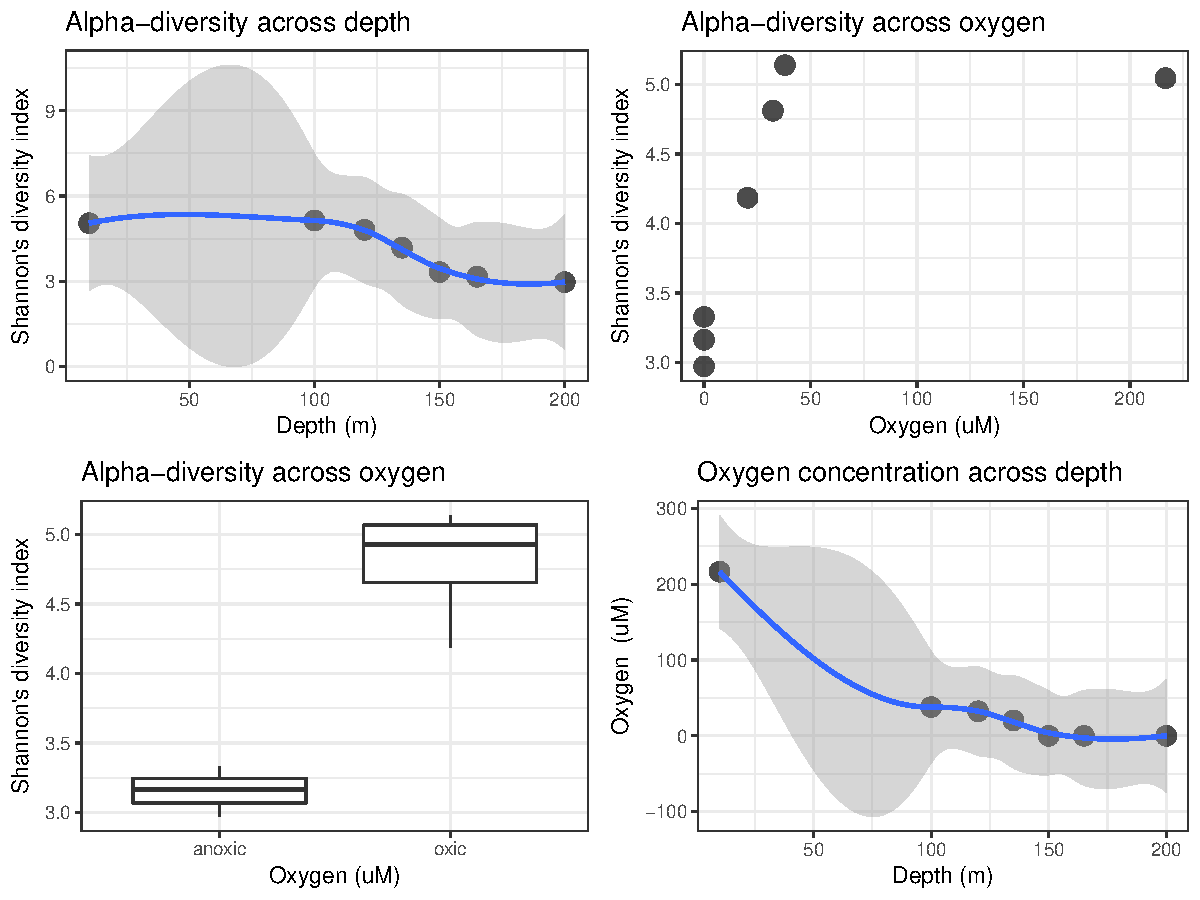
\includegraphics{Figs/unnamed-chunk-7-1.pdf}

The following function will assist us to understand the unique Phylum
rank:

\begin{Shaded}
\begin{Highlighting}[]
\KeywordTok{get_taxa_unique}\NormalTok{(}\DataTypeTok{physeq =}\NormalTok{ thirdTaxa, }\DataTypeTok{taxonomic.rank =} \StringTok{"Phylum"}\NormalTok{)}
\end{Highlighting}
\end{Shaded}

\begin{verbatim}
## [1] "Proteobacteria"                "Bacteroidetes"                
## [3] "Thaumarchaeota"                "Actinobacteria"               
## [5] "Marinimicrobia_(SAR406_clade)" "Planctomycetes"               
## [7] "Verrucomicrobia"
\end{verbatim}

We choose the \emph{Planctomycetes} phylum, and explored the
distribution of genera of this phylum.

\begin{Shaded}
\begin{Highlighting}[]
\NormalTok{subTaxa =}\StringTok{ }\KeywordTok{subset_taxa}\NormalTok{(thirdTaxa, Phylum }\OperatorTok{==}\StringTok{ "Planctomycetes"}\NormalTok{)}
\KeywordTok{plot_bar}\NormalTok{(subTaxa, }\DataTypeTok{fill =} \StringTok{"Genus"}\NormalTok{) }\OperatorTok{+}\StringTok{ }\KeywordTok{geom_bar}\NormalTok{(}\KeywordTok{aes}\NormalTok{(}\DataTypeTok{color =}\NormalTok{ Genus, }\DataTypeTok{fill =}\NormalTok{ Genus), }
    \DataTypeTok{stat =} \StringTok{"identity"}\NormalTok{, }\DataTypeTok{position =} \StringTok{"stack"}\NormalTok{) }\OperatorTok{+}\StringTok{ }\KeywordTok{labs}\NormalTok{(}\DataTypeTok{title =} \StringTok{"Genus distribution of Planctomycetes across samples"}\NormalTok{)}
\end{Highlighting}
\end{Shaded}

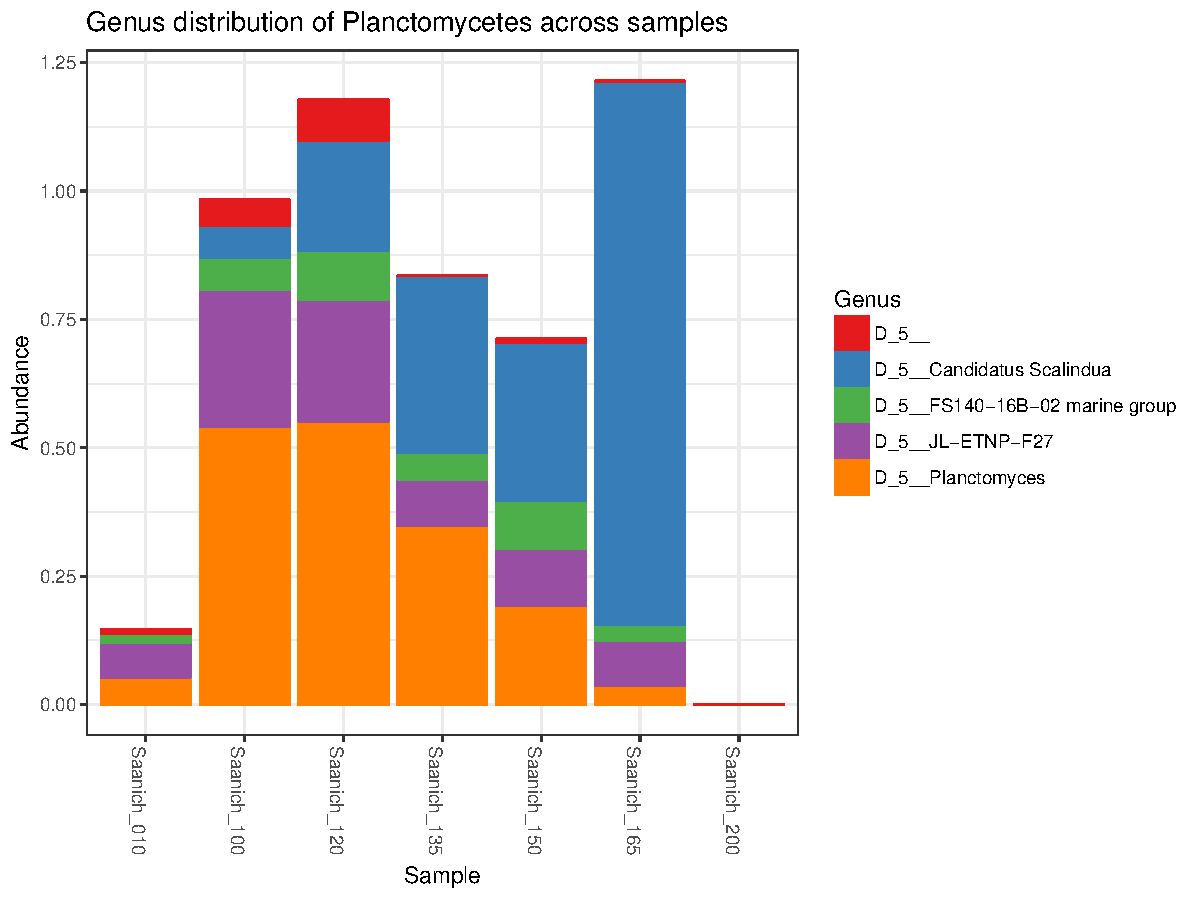
\includegraphics{Figs/unnamed-chunk-9-1.pdf}

We further investigated the genus distribution of this phylum across
samples grouped by family level.

\begin{Shaded}
\begin{Highlighting}[]
\KeywordTok{plot_bar}\NormalTok{(subTaxa, }\DataTypeTok{fill =} \StringTok{"Genus"}\NormalTok{, }\DataTypeTok{facet_grid =} \OperatorTok{~}\NormalTok{Family) }\OperatorTok{+}\StringTok{ }\KeywordTok{geom_bar}\NormalTok{(}\KeywordTok{aes}\NormalTok{(}\DataTypeTok{color =}\NormalTok{ Genus, }
    \DataTypeTok{fill =}\NormalTok{ Genus), }\DataTypeTok{stat =} \StringTok{"identity"}\NormalTok{, }\DataTypeTok{position =} \StringTok{"stack"}\NormalTok{) }\OperatorTok{+}\StringTok{ }\KeywordTok{labs}\NormalTok{(}\DataTypeTok{title =} \StringTok{"Genus distribution of Planctomycetes across samples grouped by family level"}\NormalTok{)}
\end{Highlighting}
\end{Shaded}

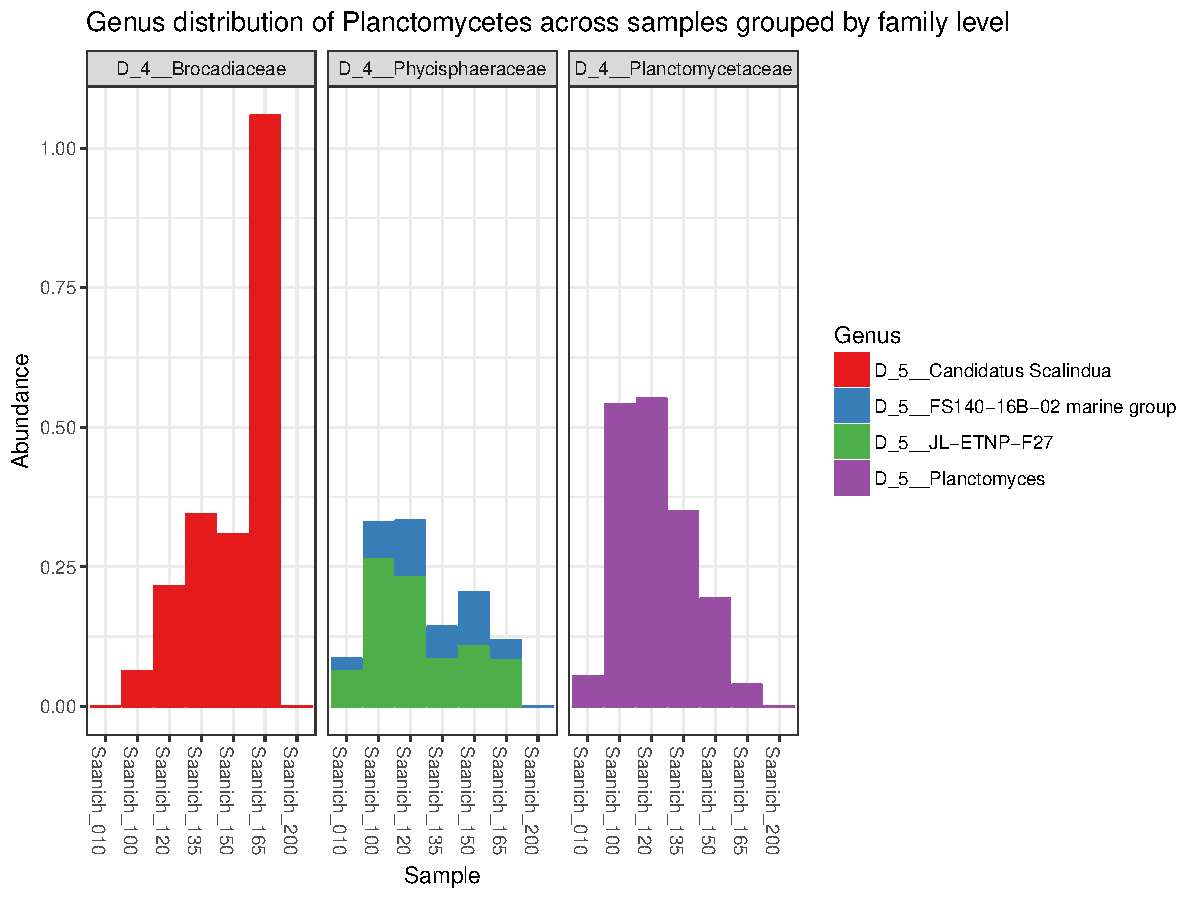
\includegraphics{Figs/unnamed-chunk-10-1.pdf}

Finally, we settled on performing experimental analysis at
\emph{Planctomyces} genus level and it's associated OTUs.

\begin{Shaded}
\begin{Highlighting}[]
\NormalTok{workingTaxa =}\StringTok{ }\KeywordTok{subset_taxa}\NormalTok{(thirdTaxa, Genus }\OperatorTok{==}\StringTok{ "Planctomyces"}\NormalTok{)}
\NormalTok{(suggestedOTUs <-}\StringTok{ }\KeywordTok{colnames}\NormalTok{(}\KeywordTok{otu_table}\NormalTok{(workingTaxa)))}
\end{Highlighting}
\end{Shaded}

\begin{verbatim}
## [1] "Otu0125" "Otu0144" "Otu0401" "Otu0592"
\end{verbatim}

\subsection{\texorpdfstring{Analysis of abundance information of
{[}OTU****{]} along with depth and/or oxygen concentration
\label{sec:OTUabundance}}{Analysis of abundance information of {[}OTU****{]} along with depth and/or oxygen concentration }}\label{analysis-of-abundance-information-of-otu-along-with-depth-andor-oxygen-concentration}

\begin{Shaded}
\begin{Highlighting}[]
\NormalTok{workingTaxa }\OperatorTok\StringTok{ }\KeywordTok{tax_glom}\NormalTok{(}\DataTypeTok{taxrank =} \StringTok{"Genus"}\NormalTok{) }\OperatorTok\StringTok{ }\KeywordTok{psmelt}\NormalTok{() }\OperatorTok\StringTok{ }\KeywordTok{lm}\NormalTok{(Abundance }\OperatorTok{~}\StringTok{ }
\StringTok{    }\NormalTok{Depth_m, .) }\OperatorTok\StringTok{ }\KeywordTok{summary}\NormalTok{()}
\end{Highlighting}
\end{Shaded}

\begin{verbatim}
## 
## Call:
## lm(formula = Abundance ~ Depth_m, data = .)
## 
## Residuals:
##        3        2        4        5        1        6        7 
##  0.19679  0.17658  0.02621 -0.06838 -0.14891 -0.09696 -0.08533 
## 
## Coefficients:
##               Estimate Std. Error t value Pr(>|t|)
## (Intercept)  0.1575152  0.1406836   1.120    0.314
## Depth_m     -0.0003609  0.0010227  -0.353    0.739
## 
## Residual standard error: 0.1511 on 5 degrees of freedom
## Multiple R-squared:  0.0243, Adjusted R-squared:  -0.1708 
## F-statistic: 0.1245 on 1 and 5 DF,  p-value: 0.7386
\end{verbatim}

\begin{Shaded}
\begin{Highlighting}[]
\NormalTok{workingTaxa }\OperatorTok\StringTok{ }\KeywordTok{psmelt}\NormalTok{() }\OperatorTok\StringTok{ }\KeywordTok{group_by}\NormalTok{(Sample) }\OperatorTok\StringTok{ }\KeywordTok{summarize}\NormalTok{(}\DataTypeTok{Abundance_sum =} \KeywordTok{sum}\NormalTok{(Abundance), }
    \DataTypeTok{Depth_m =} \KeywordTok{mean}\NormalTok{(Depth_m)) }\OperatorTok\StringTok{ }\KeywordTok{ggplot}\NormalTok{() }\OperatorTok{+}\StringTok{ }\KeywordTok{geom_point}\NormalTok{(}\KeywordTok{aes}\NormalTok{(}\DataTypeTok{x =}\NormalTok{ Depth_m, }\DataTypeTok{y =}\NormalTok{ Abundance_sum), }
    \DataTypeTok{size =} \DecValTok{5}\NormalTok{, }\DataTypeTok{alpha =} \FloatTok{0.7}\NormalTok{) }\OperatorTok{+}\StringTok{ }\KeywordTok{geom_smooth}\NormalTok{(}\DataTypeTok{method =} \StringTok{"lm"}\NormalTok{, }\KeywordTok{aes}\NormalTok{(}\DataTypeTok{x =} \KeywordTok{as.numeric}\NormalTok{(Depth_m), }
    \DataTypeTok{y =}\NormalTok{ Abundance_sum)) }\OperatorTok{+}\StringTok{ }\KeywordTok{labs}\NormalTok{(}\DataTypeTok{title =} \StringTok{"Abundance of Plantomyces across depth"}\NormalTok{)}
\end{Highlighting}
\end{Shaded}

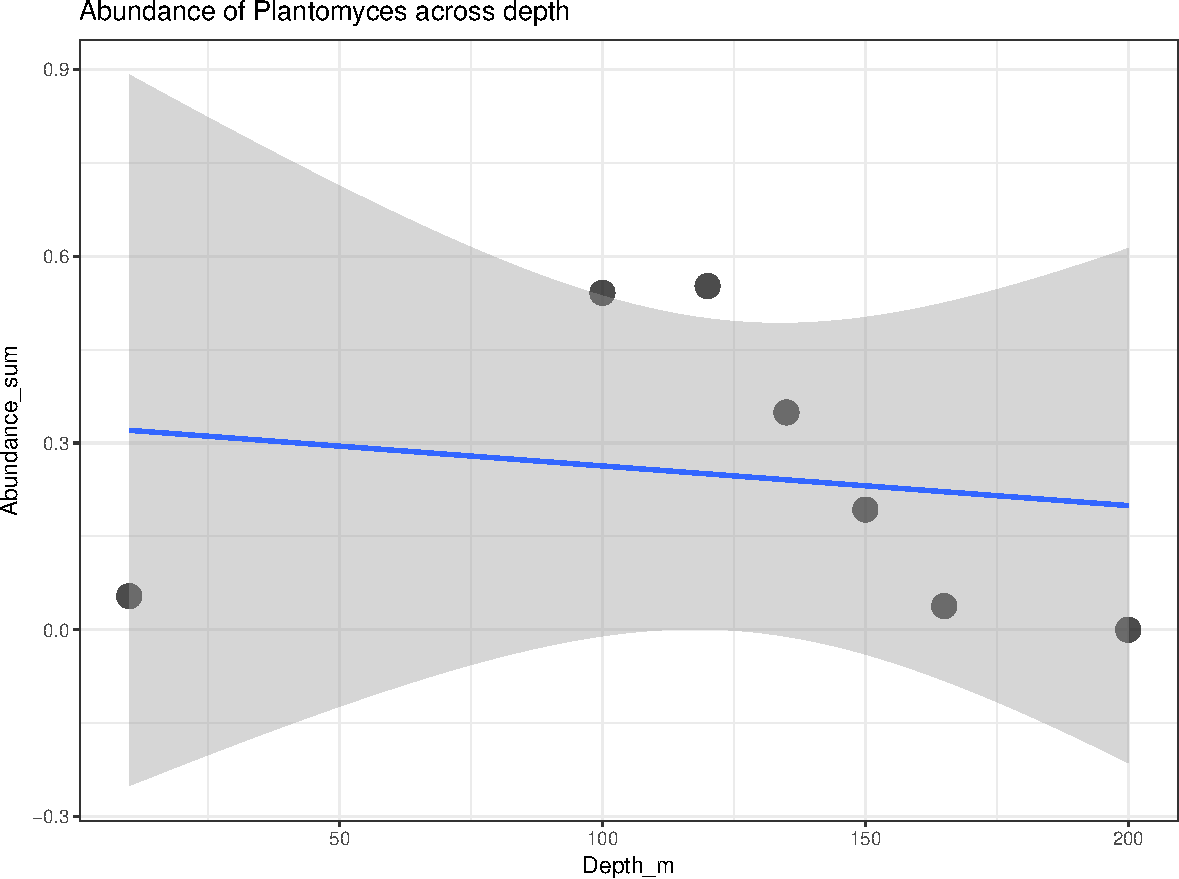
\includegraphics{Figs/unnamed-chunk-12-1.pdf}

\begin{Shaded}
\begin{Highlighting}[]
\NormalTok{workingTaxa }\OperatorTok\StringTok{ }\KeywordTok{tax_glom}\NormalTok{(}\DataTypeTok{taxrank =} \StringTok{"Genus"}\NormalTok{) }\OperatorTok\StringTok{ }\KeywordTok{psmelt}\NormalTok{() }\OperatorTok\StringTok{ }\KeywordTok{lm}\NormalTok{(Abundance }\OperatorTok{~}\StringTok{ }
\StringTok{    }\NormalTok{O2_uM, .) }\OperatorTok\StringTok{ }\KeywordTok{summary}\NormalTok{()}
\end{Highlighting}
\end{Shaded}

\begin{verbatim}
## 
## Call:
## lm(formula = Abundance ~ O2_uM, data = .)
## 
## Residuals:
##        3        2        4        5        1        6        7 
##  0.19591  0.18435  0.01688 -0.08832 -0.06319 -0.12232 -0.12332 
## 
## Coefficients:
##               Estimate Std. Error t value Pr(>|t|)
## (Intercept)  0.1233192  0.0670191    1.84    0.125
## O2_uM       -0.0002544  0.0007941   -0.32    0.762
## 
## Residual standard error: 0.1514 on 5 degrees of freedom
## Multiple R-squared:  0.02012,    Adjusted R-squared:  -0.1759 
## F-statistic: 0.1027 on 1 and 5 DF,  p-value: 0.7616
\end{verbatim}

\begin{Shaded}
\begin{Highlighting}[]
\NormalTok{workingTaxa }\OperatorTok\StringTok{ }\KeywordTok{psmelt}\NormalTok{() }\OperatorTok\StringTok{ }\KeywordTok{group_by}\NormalTok{(Sample) }\OperatorTok\StringTok{ }\KeywordTok{summarize}\NormalTok{(}\DataTypeTok{Abundance_sum =} \KeywordTok{sum}\NormalTok{(Abundance), }
    \DataTypeTok{Oxyzen =} \KeywordTok{mean}\NormalTok{(O2_uM)) }\OperatorTok\StringTok{ }\KeywordTok{ggplot}\NormalTok{() }\OperatorTok{+}\StringTok{ }\KeywordTok{geom_point}\NormalTok{(}\KeywordTok{aes}\NormalTok{(}\DataTypeTok{x =}\NormalTok{ Oxyzen, }\DataTypeTok{y =}\NormalTok{ Abundance_sum), }
    \DataTypeTok{size =} \DecValTok{5}\NormalTok{, }\DataTypeTok{alpha =} \FloatTok{0.7}\NormalTok{) }\OperatorTok{+}\StringTok{ }\KeywordTok{geom_smooth}\NormalTok{(}\DataTypeTok{method =} \StringTok{"lm"}\NormalTok{, }\KeywordTok{aes}\NormalTok{(}\DataTypeTok{x =} \KeywordTok{as.numeric}\NormalTok{(Oxyzen), }
    \DataTypeTok{y =}\NormalTok{ Abundance_sum)) }\OperatorTok{+}\StringTok{ }\KeywordTok{labs}\NormalTok{(}\DataTypeTok{title =} \StringTok{"Abundance of Plantomyces with respect to oxyzen concentration"}\NormalTok{)}
\end{Highlighting}
\end{Shaded}

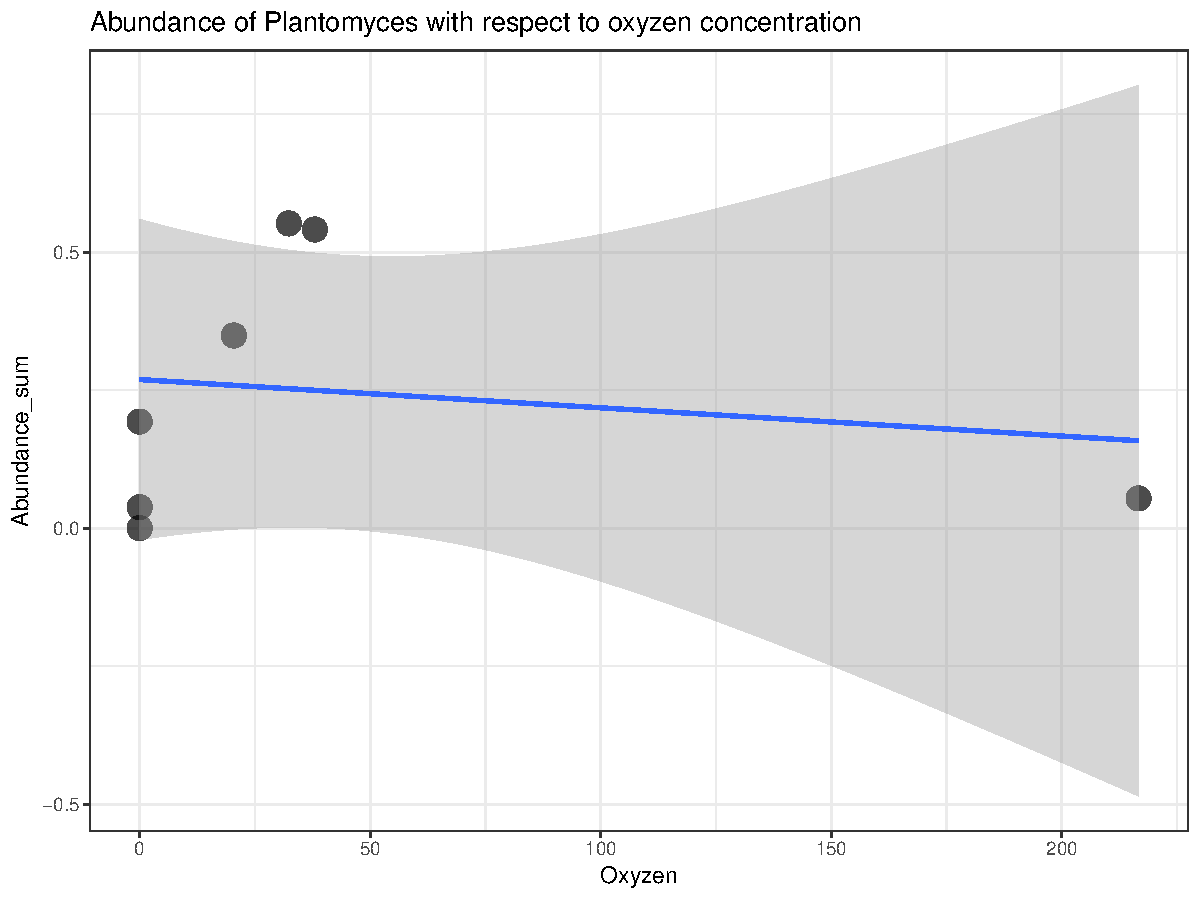
\includegraphics{Figs/unnamed-chunk-13-1.pdf}

\subsection{\texorpdfstring{Estimate richness (number of OTUs/ASVs) for
{[}OTU****{]}
\label{sec:richness}}{Estimate richness (number of OTUs/ASVs) for {[}OTU****{]} }}\label{estimate-richness-number-of-otusasvs-for-otu}

We explore the diversity of \emph{Planctomyces} across depth.

\begin{Shaded}
\begin{Highlighting}[]
\NormalTok{workingTaxa }\OperatorTok\StringTok{ }\KeywordTok{plot_richness}\NormalTok{(}\DataTypeTok{x =} \StringTok{"Depth_m"}\NormalTok{, }\DataTypeTok{measures =} \StringTok{"Shannon"}\NormalTok{) }\OperatorTok{+}\StringTok{ }\KeywordTok{geom_smooth}\NormalTok{(}\DataTypeTok{method =} \StringTok{"loess"}\NormalTok{, }
    \KeywordTok{aes}\NormalTok{(}\DataTypeTok{x =} \KeywordTok{as.numeric}\NormalTok{(Depth_m))) }\OperatorTok{+}\StringTok{ }\KeywordTok{geom_point}\NormalTok{(}\DataTypeTok{size =} \DecValTok{5}\NormalTok{, }\DataTypeTok{alpha =} \FloatTok{0.7}\NormalTok{) }\OperatorTok{+}\StringTok{ }\KeywordTok{labs}\NormalTok{(}\DataTypeTok{title =} \StringTok{"Alpha-diversity of Plantomyces across depth"}\NormalTok{, }
    \DataTypeTok{y =} \StringTok{"Shannon's diversity index"}\NormalTok{, }\DataTypeTok{x =} \StringTok{"Depth (m)"}\NormalTok{)}
\end{Highlighting}
\end{Shaded}

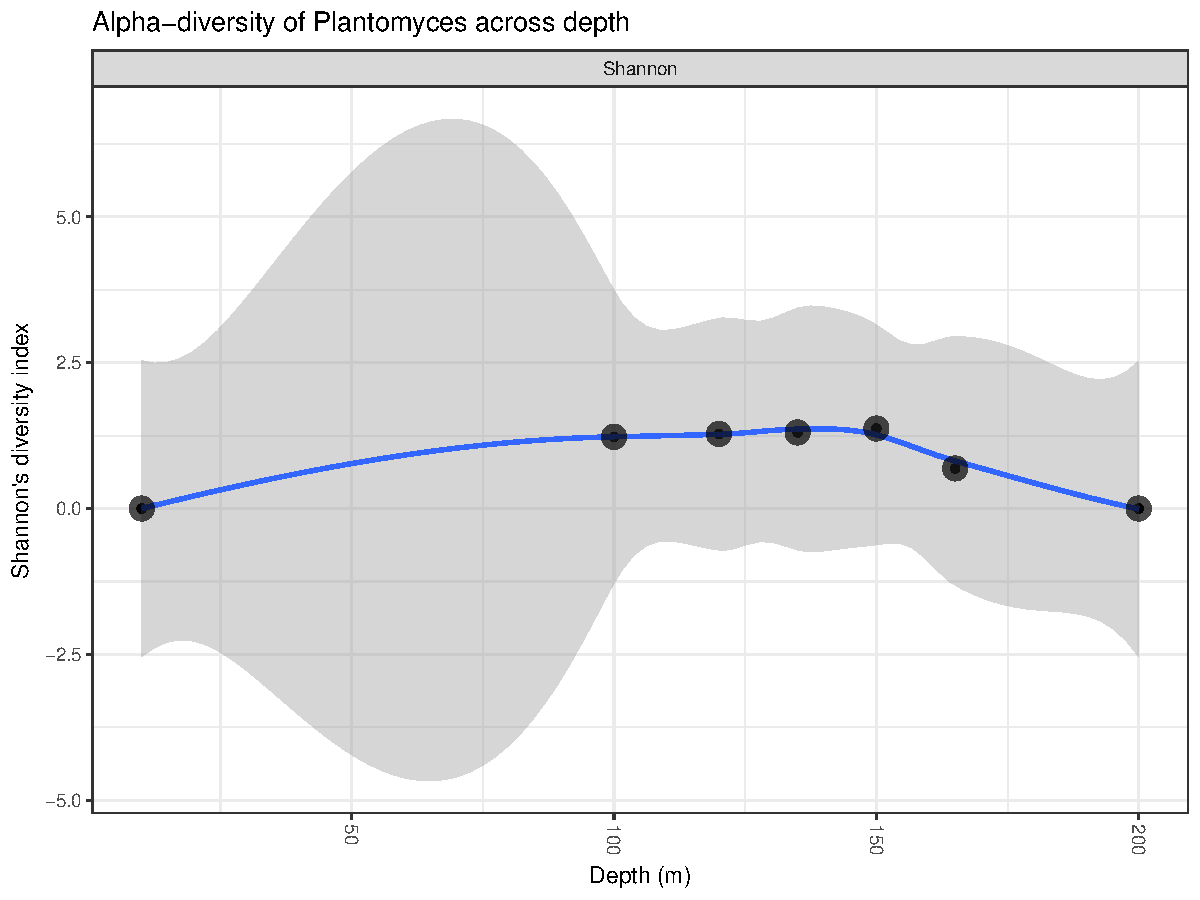
\includegraphics{Figs/unnamed-chunk-14-1.pdf}

\subsection{\texorpdfstring{Interpretation of abundance information of
OTUs/ASVs of {[}OTU****{]} along with depth and/or oxygen concentration
\label{sec:ASVabundances}}{Interpretation of abundance information of OTUs/ASVs of {[}OTU****{]} along with depth and/or oxygen concentration }}\label{interpretation-of-abundance-information-of-otusasvs-of-otu-along-with-depth-andor-oxygen-concentration}

\begin{Shaded}
\begin{Highlighting}[]
\CommentTok{# Generalized linear model for each OTU}
\ControlFlowTok{for}\NormalTok{ (otu }\ControlFlowTok{in}\NormalTok{ suggestedOTUs) \{}
    \KeywordTok{cat}\NormalTok{(}\StringTok{"### Generalized linear model for "}\NormalTok{, otu)}
\NormalTok{    workingTaxa }\OperatorTok\StringTok{ }\KeywordTok{psmelt}\NormalTok{() }\OperatorTok\StringTok{ }\KeywordTok{filter}\NormalTok{(OTU }\OperatorTok{==}\StringTok{ }\NormalTok{otu) }\OperatorTok\StringTok{ }\KeywordTok{lm}\NormalTok{(Abundance }\OperatorTok{~}\StringTok{ }\NormalTok{Depth_m, }
\NormalTok{        .) }\OperatorTok\StringTok{ }\KeywordTok{summary}\NormalTok{() }\OperatorTok\StringTok{ }\KeywordTok{print}\NormalTok{()}
\NormalTok{\}}
\end{Highlighting}
\end{Shaded}

\begin{verbatim}
## ### Generalized linear model for  Otu0125
## Call:
## lm(formula = Abundance ~ Depth_m, data = .)
## 
## Residuals:
##         1         2         3         4         5         6         7 
##  0.101457  0.100546  0.009613 -0.037320 -0.079944 -0.050254 -0.044098 
## 
## Coefficients:
##               Estimate Std. Error t value Pr(>|t|)
## (Intercept)  0.0849882  0.0753618   1.128    0.311
## Depth_m     -0.0002045  0.0005479  -0.373    0.724
## 
## Residual standard error: 0.08093 on 5 degrees of freedom
## Multiple R-squared:  0.0271, Adjusted R-squared:  -0.1675 
## F-statistic: 0.1393 on 1 and 5 DF,  p-value: 0.7243
## 
## ### Generalized linear model for  Otu0144
## Call:
## lm(formula = Abundance ~ Depth_m, data = .)
## 
## Residuals:
##        1        2        3        4        5        6        7 
##  0.07920  0.06727  0.01157 -0.02814 -0.05959 -0.03784 -0.03247 
## 
## Coefficients:
##               Estimate Std. Error t value Pr(>|t|)
## (Intercept)  0.0631237  0.0554978   1.137    0.307
## Depth_m     -0.0001533  0.0004035  -0.380    0.720
## 
## Residual standard error: 0.0596 on 5 degrees of freedom
## Multiple R-squared:  0.02805,    Adjusted R-squared:  -0.1663 
## F-statistic: 0.1443 on 1 and 5 DF,  p-value: 0.7197
## 
## ### Generalized linear model for  Otu0401
## Call:
## lm(formula = Abundance ~ Depth_m, data = .)
## 
## Residuals:
##          1          2          3          4          5          6 
##  2.399e-02  8.511e-06 -9.777e-04 -5.024e-03 -6.106e-03 -5.964e-03 
##          7 
## -5.932e-03 
## 
## Coefficients:
##               Estimate Std. Error t value Pr(>|t|)
## (Intercept)  6.115e-03  1.110e-02   0.551    0.605
## Depth_m     -9.165e-07  8.067e-05  -0.011    0.991
## 
## Residual standard error: 0.01192 on 5 degrees of freedom
## Multiple R-squared:  2.582e-05,  Adjusted R-squared:   -0.2 
## F-statistic: 0.0001291 on 1 and 5 DF,  p-value: 0.9914
## 
## ### Generalized linear model for  Otu0592
## Call:
## lm(formula = Abundance ~ Depth_m, data = .)
## 
## Residuals:
##          1          2          3          4          5          6 
##  0.0049869  0.0050213  0.0009411 -0.0019444 -0.0032651 -0.0029100 
##          7 
## -0.0028298 
## 
## Coefficients:
##               Estimate Std. Error t value Pr(>|t|)
## (Intercept)  3.288e-03  3.768e-03   0.873    0.423
## Depth_m     -2.291e-06  2.740e-05  -0.084    0.937
## 
## Residual standard error: 0.004047 on 5 degrees of freedom
## Multiple R-squared:  0.001397,   Adjusted R-squared:  -0.1983 
## F-statistic: 0.006996 on 1 and 5 DF,  p-value: 0.9366
\end{verbatim}

\begin{Shaded}
\begin{Highlighting}[]
\KeywordTok{p.adjust}\NormalTok{(}\KeywordTok{runif}\NormalTok{(}\KeywordTok{length}\NormalTok{(suggestedOTUs), }\DataTypeTok{min =} \FloatTok{0.005}\NormalTok{, }\DataTypeTok{max =} \FloatTok{0.85}\NormalTok{), }\DataTypeTok{method =} \StringTok{"fdr"}\NormalTok{)}
\end{Highlighting}
\end{Shaded}

\begin{verbatim}
## [1] 0.5484101 0.5484101 0.5484101 0.5484101
\end{verbatim}

\begin{Shaded}
\begin{Highlighting}[]
\CommentTok{# Abundance of OTUs within unclassified domain across depth}
\NormalTok{p5 <-}\StringTok{ }\NormalTok{workingTaxa }\OperatorTok\StringTok{ }\KeywordTok{psmelt}\NormalTok{() }\OperatorTok\StringTok{ }\KeywordTok{ggplot}\NormalTok{() }\OperatorTok{+}\StringTok{ }\KeywordTok{geom_point}\NormalTok{(}\KeywordTok{aes}\NormalTok{(}\DataTypeTok{x =}\NormalTok{ Depth_m, }\DataTypeTok{y =}\NormalTok{ Abundance), }
    \DataTypeTok{size =} \DecValTok{5}\NormalTok{, }\DataTypeTok{alpha =} \FloatTok{0.7}\NormalTok{) }\OperatorTok{+}\StringTok{ }\KeywordTok{geom_smooth}\NormalTok{(}\DataTypeTok{method =} \StringTok{"lm"}\NormalTok{, }\KeywordTok{aes}\NormalTok{(}\DataTypeTok{x =}\NormalTok{ Depth_m, }\DataTypeTok{y =}\NormalTok{ Abundance)) }\OperatorTok{+}\StringTok{ }
\StringTok{    }\KeywordTok{facet_wrap}\NormalTok{(}\OperatorTok{~}\NormalTok{OTU, }\DataTypeTok{scales =} \StringTok{"free_y"}\NormalTok{) }\OperatorTok{+}\StringTok{ }\KeywordTok{labs}\NormalTok{(}\DataTypeTok{title =} \StringTok{"Abundance of OTUs within Planctomyces genus across depth"}\NormalTok{)}

\CommentTok{# Abundance of OTUs within unclassified depth by colour}
\NormalTok{p6 <-}\StringTok{ }\NormalTok{workingTaxa }\OperatorTok\StringTok{ }\KeywordTok{psmelt}\NormalTok{() }\OperatorTok\StringTok{ }\KeywordTok{ggplot}\NormalTok{() }\OperatorTok{+}\StringTok{ }\KeywordTok{geom_point}\NormalTok{(}\KeywordTok{aes}\NormalTok{(}\DataTypeTok{x =}\NormalTok{ Sample, }\DataTypeTok{y =}\NormalTok{ OTU, }
    \DataTypeTok{size =}\NormalTok{ Abundance, }\DataTypeTok{color =}\NormalTok{ OTU)) }\OperatorTok{+}\StringTok{ }\KeywordTok{scale_size_continuous}\NormalTok{(}\DataTypeTok{range =} \KeywordTok{c}\NormalTok{(}\DecValTok{0}\NormalTok{, }\DecValTok{5}\NormalTok{)) }\OperatorTok{+}\StringTok{ }
\StringTok{    }\KeywordTok{labs}\NormalTok{(}\DataTypeTok{title =} \StringTok{"Abundance of OTUs within Planctomyces genus across depth"}\NormalTok{)}

\KeywordTok{grid.arrange}\NormalTok{(p5, p6, }\DataTypeTok{ncol =} \DecValTok{2}\NormalTok{)}
\end{Highlighting}
\end{Shaded}

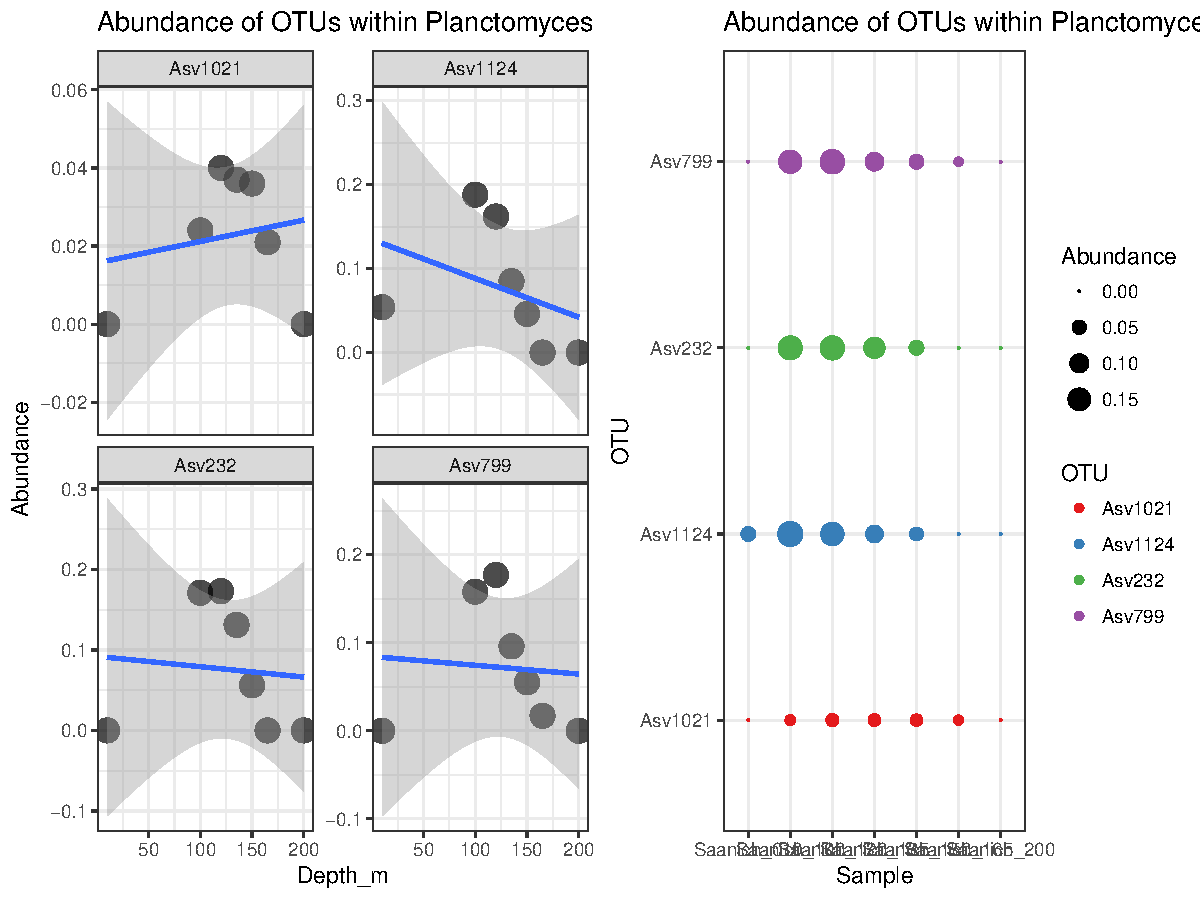
\includegraphics{Figs/unnamed-chunk-16-1.pdf}

\begin{Shaded}
\begin{Highlighting}[]
\CommentTok{# Abundance of OTUs within Planctomyces genus across depth}
\NormalTok{p7 <-}\StringTok{ }\NormalTok{workingTaxa }\OperatorTok\StringTok{ }\KeywordTok{psmelt}\NormalTok{() }\OperatorTok\StringTok{ }\KeywordTok{ggplot}\NormalTok{() }\OperatorTok{+}\StringTok{ }\KeywordTok{geom_point}\NormalTok{(}\KeywordTok{aes}\NormalTok{(}\DataTypeTok{x =}\NormalTok{ O2_uM, }\DataTypeTok{y =}\NormalTok{ Abundance), }
    \DataTypeTok{size =} \DecValTok{5}\NormalTok{, }\DataTypeTok{alpha =} \FloatTok{0.7}\NormalTok{) }\OperatorTok{+}\StringTok{ }\KeywordTok{geom_smooth}\NormalTok{(}\DataTypeTok{method =} \StringTok{"lm"}\NormalTok{, }\KeywordTok{aes}\NormalTok{(}\DataTypeTok{x =}\NormalTok{ O2_uM, }\DataTypeTok{y =}\NormalTok{ Abundance)) }\OperatorTok{+}\StringTok{ }
\StringTok{    }\KeywordTok{facet_wrap}\NormalTok{(}\OperatorTok{~}\NormalTok{OTU, }\DataTypeTok{scales =} \StringTok{"free_y"}\NormalTok{) }\OperatorTok{+}\StringTok{ }\KeywordTok{labs}\NormalTok{(}\DataTypeTok{title =} \StringTok{"Abundance of OTUs within Planctomyces genus across oxygen concentration"}\NormalTok{)}

\CommentTok{# Abundance of OTUs within Planctomyces genus by colour}
\NormalTok{p8 <-}\StringTok{ }\NormalTok{workingTaxa }\OperatorTok\StringTok{ }\KeywordTok{psmelt}\NormalTok{() }\OperatorTok\StringTok{ }\KeywordTok{ggplot}\NormalTok{() }\OperatorTok{+}\StringTok{ }\KeywordTok{geom_point}\NormalTok{(}\KeywordTok{aes}\NormalTok{(}\DataTypeTok{x =}\NormalTok{ Sample, }\DataTypeTok{y =}\NormalTok{ OTU, }
    \DataTypeTok{size =}\NormalTok{ O2_uM, }\DataTypeTok{color =}\NormalTok{ OTU)) }\OperatorTok{+}\StringTok{ }\KeywordTok{scale_size_continuous}\NormalTok{(}\DataTypeTok{range =} \KeywordTok{c}\NormalTok{(}\DecValTok{0}\NormalTok{, }\DecValTok{5}\NormalTok{)) }\OperatorTok{+}\StringTok{ }\KeywordTok{labs}\NormalTok{(}\DataTypeTok{title =} \StringTok{"Abundance of OTUs within Planctomyces genus across oxygen concentration"}\NormalTok{)}

\KeywordTok{grid.arrange}\NormalTok{(p7, p8, }\DataTypeTok{ncol =} \DecValTok{2}\NormalTok{)}
\end{Highlighting}
\end{Shaded}

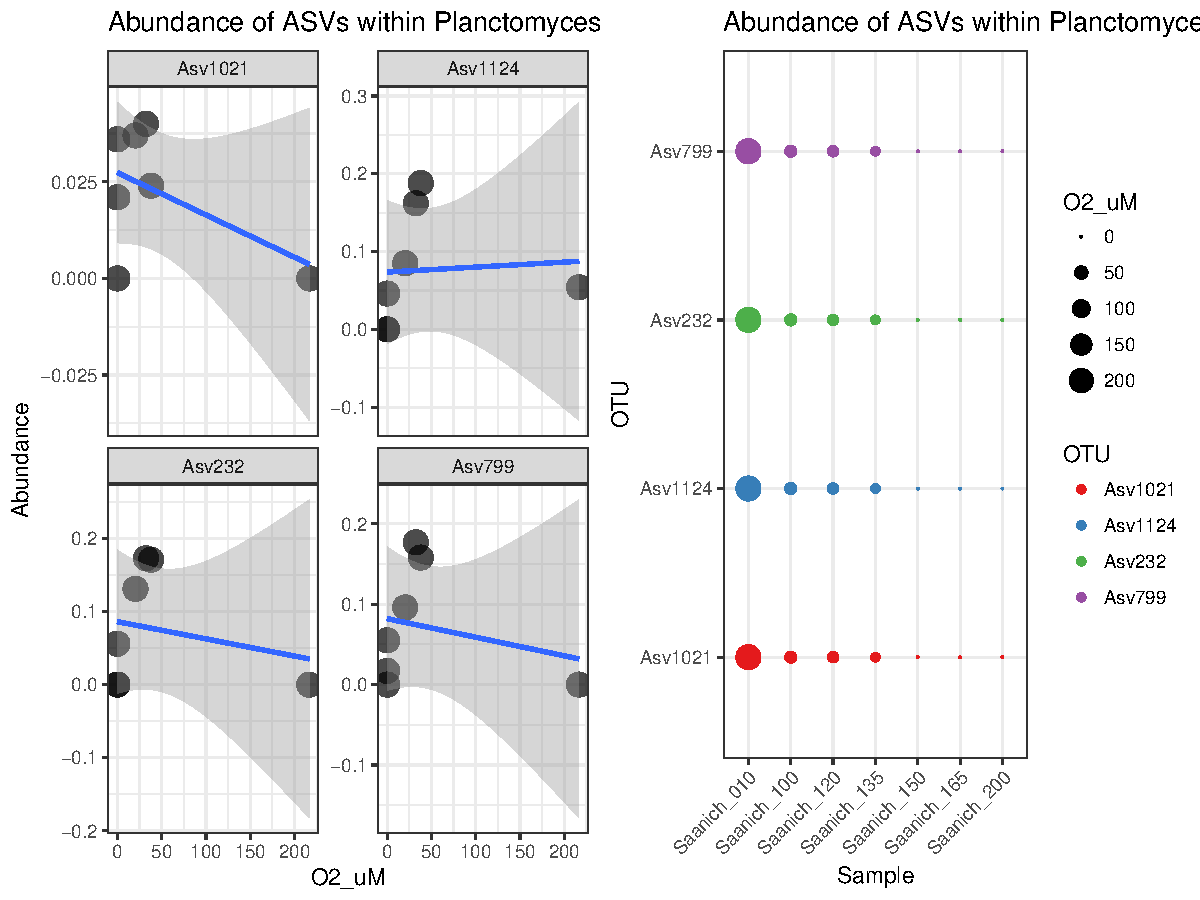
\includegraphics{Figs/unnamed-chunk-17-1.pdf}

\section{Discussion}\label{discussion}

(Hawley et al. 2017; Torres-Beltrán et al. 2017)

\begin{center}\rule{0.5\linewidth}{\linethickness}\end{center}

\section*{References}\label{references}
\addcontentsline{toc}{section}{References}

\hypertarget{refs}{}
\hypertarget{ref-Hawley2017:compendium}{}
Hawley, Alyse K, Mónica Torres-Beltrán, Elena Zaikova, David A Walsh,
Andreas Mueller, Melanie Scofield, Sam Kheirandish, et al. 2017. ``A
Compendium of Multi-Omic Sequence Information from the Saanich Inlet
Water Column.'' \emph{Scientific Data} 4. Nature Publishing Group:
170160.

\hypertarget{ref-Torres2017:compendium}{}
Torres-Beltrán, Mónica, Alyse K Hawley, David Capelle, Elena Zaikova,
David A Walsh, Andreas Mueller, Melanie Scofield, et al. 2017. ``A
Compendium of Geochemical Information from the Saanich Inlet Water
Column.'' \emph{Scientific Data} 4. Nature Publishing Group: 170159.


\end{document}
